\chapter{Configure Settings}

When connected, the other menues will become available. In the 'configure settings' menu, there are several options that must be specified, however default values are provided:
You can see the window below: \\
    \begin{figure}[H]
        \centering
        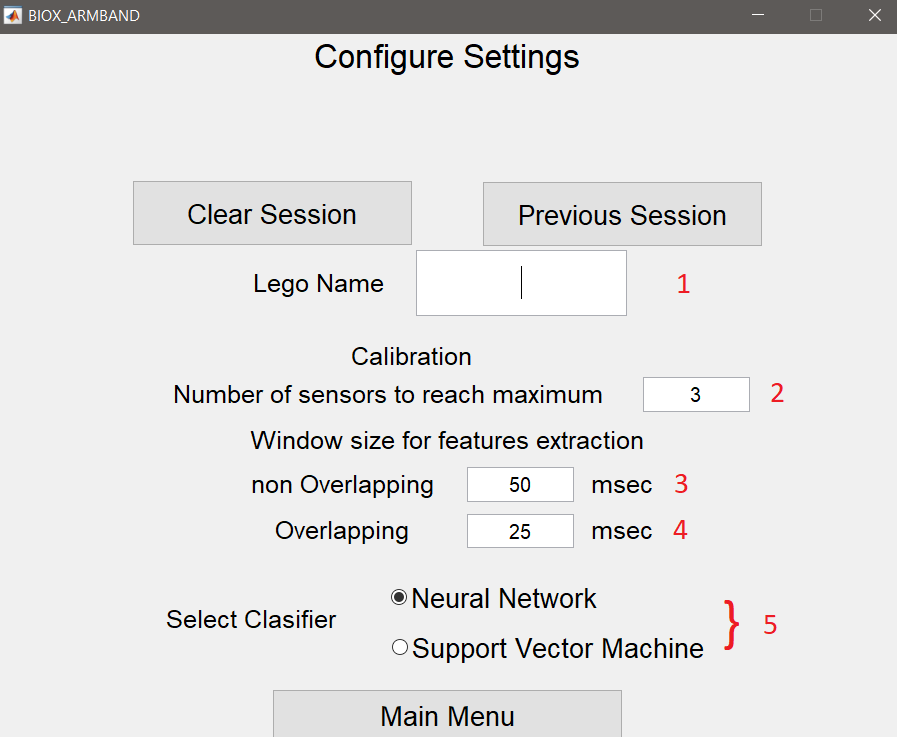
\includegraphics[width=0.6\linewidth]{figures/AppPics/2_Configure_settings_NEW.png}
        \caption{Configure settings menu.}
        \label{fig:my_label}
    \end{figure}

\begin{enumerate}[label=\textbf{Step \arabic*}:]
    \item The name of the LEGO Mindstorm unit must be entered, if you wish to use such device. This is done in setting \textcolor{red}{"1"}. (Note that the input is case sensitive).
    \item Next, specify the number of sensors that must be amplified to reach maximum range. This is done in setting \textcolor{red}{"2"}.
    \item Now specify the the non-overlapping sample window interval in milliseconds (or number of samples). This is recommended to be \textbf{bewteen 25 ms and 500 ms}. Note that this is a trade-off between accuracy and responsiveness; the lower the value the faster response time, but less accuracy. Fill out setting \textcolor{red}{"3"} to achieve this.
    \item Specify overlapping sample window interval in milliseconds (or number of samples). This is the amount of time (or samples) taken from previous window and added to the next, to ensure consistency. This is done in setting \textcolor{red}{"4"}.
    \item Lastly, choose the desired classifier in setting \textcolor{red}{"5"}.
    \item If settings from a previous session is required, click the \textbf{"Previous Session"} button and locate the settings-file. If this file contains calibration and training data aswell, then these two steps can be skipped in the main menu and testing can begin immediately.
    \item Click \textbf{"Main Menu"} to return to the main menu.
\end{enumerate}